\chapter{Introducción}

\section{Contexto}
Esta aplicación va a estar orientada a hacer de soporte a deportistas, tanto experimentados como no.
Un ejercicio, es la repetición de un movimiento varias veces para estimular uno o varios músculos.
Los entrenamientos, entendámolos como la colección de distintos ejercicios destinados a entrenar una parte o varias del cuerpo.
Una serie, es cuando dentro de un ejercicio, repetimos ese movimiento un número determinado de veces y se realiza un descanso, sin cambiar de ejercicio.
Una repetición, es la realización del movimiento de ese ejercicio en una serie, es decir, si estoy haciendo flexiones, hago 12, descanso, hago 10, descanso, hago 9 y ya no hago más flexiones, dentro de mi entrenamiento se vería así:


\underline {Rutina de entrenamiento 1:}
\begin{itemize}
	\item Ejercicio 1
	\begin{itemize}
		\item Serie 1: X repeticiones
		\item Serie 2: X repeticiones
	\end{itemize}
	\item Flexiones
	\begin{itemize}
		\item Serie 1: 12 repeticiones
		\item Serie 2: 10 repeticiones 
		\item Serie 3: 9 repeticiones
	\end{itemize}
	\item Ejercicio 3
	\begin{itemize}
		\item Serie 1: X repeticiones
		\item Serie 2: X repeticiones
	\end{itemize}
\end{itemize}

\section{Justificación y Motivación}
Algunas de las aplicaciones que existen, para mediciones de constantes relacionadas durante el entrenamiento físico, suelen ser de pago. Ejemplos:
\begin{itemize}
	\item MyFitnessPal: €9.99
	\item Whoop: €28
	\item Fitbit Premium: €9.99
	\item Apple Fitness+: €9.99
	\item Strava Premium: €5.99
\end{itemize}

Es verdad que algunas tienen versión gratuita, pero no ofrecen la totalidad de sus funcionalidades, de hecho, estas versiones suelen ser extremadamente limitadas. Otras aplicaciones como Garmin Connect, si que son gratuitas, pero te obligan a ceñirte a un smartwatch de la marca Garmin, los cuales su precio no baja de los 300€.

La app que estoy presentando daría la mayoría de funcionalidades de pago de una manera más barata que el resto y aporta su funcionalidad de medir de forma personalizada el rendimiento del deportista. También se añade la IA que permite aconsejar al usuario.

Aquí una tabla resumiendo funcionalidades:
\begin{figure}[h!]
  \centering
  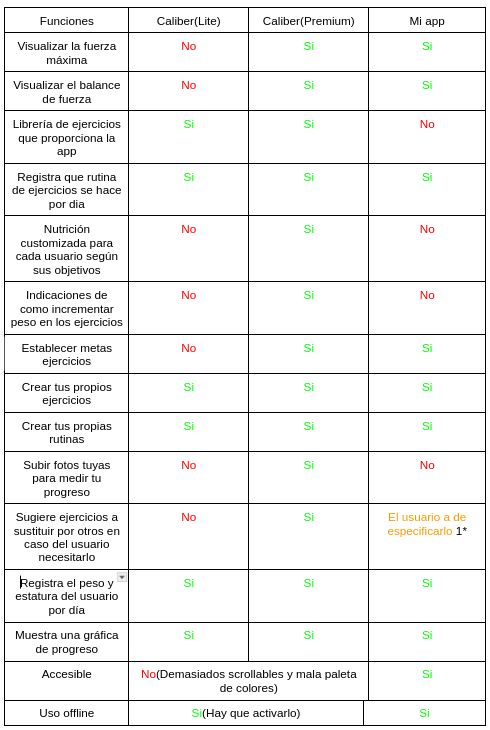
\includegraphics[width=0.7\textwidth]{tablas/comparativa.png}
  \caption{Descripción de la imagen}
  \label{fig:imagen}
\end{figure}
\newpage

\documentclass{article}
\usepackage{amsmath}
\usepackage{color,pxfonts,fix-cm}
\usepackage{latexsym}
\usepackage[mathletters]{ucs}
\DeclareUnicodeCharacter{32}{$\ $}
\usepackage[ArialMT,T1]{fontenc}
\usepackage[utf8x]{inputenc}
\usepackage{pict2e}
\usepackage{wasysym}
\usepackage[english]{babel}
\usepackage{tikz}
\pagestyle{empty}
\usepackage[margin=0in,paperwidth=595pt,paperheight=841pt]{geometry}
\begin{document}
\definecolor{color_29791}{rgb}{0,0,0}
\definecolor{color_274846}{rgb}{1,0,0}
\definecolor{color_37696}{rgb}{0,1,0}
\definecolor{color_279589}{rgb}{1,0.6,0}
\begin{tikzpicture}[overlay]\path(0pt,0pt);\end{tikzpicture}
\begin{picture}(-5,0)(2.5,0)
\put(90.35,-91.91101){\fontsize{11}{1}\selectfont\color{color_29791}Funciones}
\put(200.1,-91.91101){\fontsize{11}{1}\selectfont\color{color_29791}Caliber(Lite)}
\put(299.5,-91.91101){\fontsize{11}{1}\selectfont\color{color_29791}Caliber(Premium)}
\put(437.45,-91.91101){\fontsize{11}{1}\selectfont\color{color_29791}Mi app}
\put(69.25,-115.561){\fontsize{11}{1}\selectfont\color{color_29791}Visualizar la fuerza}
\put(162.2,-115.561){\fontsize{11}{1}\selectfont\color{color_29791} }
\put(96.45,-128.211){\fontsize{11}{1}\selectfont\color{color_29791}máxima}
\put(223.05,-115.561){\fontsize{11}{1}\selectfont\color{color_274846}No}
\put(337.7,-115.561){\fontsize{11}{1}\selectfont\color{color_37696}Si}
\put(449.05,-115.561){\fontsize{11}{1}\selectfont\color{color_37696}Si}
\put(65.25,-151.861){\fontsize{11}{1}\selectfont\color{color_29791}Visualizar el balance}
\put(166.15,-151.861){\fontsize{11}{1}\selectfont\color{color_29791} }
\put(92.8,-164.511){\fontsize{11}{1}\selectfont\color{color_29791}de fuerza}
\put(223.05,-151.861){\fontsize{11}{1}\selectfont\color{color_274846}No}
\put(337.7,-151.861){\fontsize{11}{1}\selectfont\color{color_37696}Si}
\put(449.05,-151.861){\fontsize{11}{1}\selectfont\color{color_37696}Si}
\put(64.95,-188.161){\fontsize{11}{1}\selectfont\color{color_29791}Librería de ejercicios}
\put(166.45,-188.161){\fontsize{11}{1}\selectfont\color{color_29791} }
\put(70.15,-200.811){\fontsize{11}{1}\selectfont\color{color_29791}que proporciona la}
\put(161.25,-200.811){\fontsize{11}{1}\selectfont\color{color_29791} }
\put(106.55,-213.461){\fontsize{11}{1}\selectfont\color{color_29791}app}
\put(225.15,-188.161){\fontsize{11}{1}\selectfont\color{color_37696}Si}
\put(337.7,-188.161){\fontsize{11}{1}\selectfont\color{color_37696}Si}
\put(446.95,-188.161){\fontsize{11}{1}\selectfont\color{color_274846}No}
\put(69.25,-237.111){\fontsize{11}{1}\selectfont\color{color_29791}Registra que rutina}
\put(162.2,-237.111){\fontsize{11}{1}\selectfont\color{color_29791} }
\put(64.35,-249.761){\fontsize{11}{1}\selectfont\color{color_29791}de ejercicios se hace}
\put(167.05,-249.761){\fontsize{11}{1}\selectfont\color{color_29791} }
\put(98.9,-262.411){\fontsize{11}{1}\selectfont\color{color_29791}por dia}
\put(225.15,-237.111){\fontsize{11}{1}\selectfont\color{color_37696}Si}
\put(337.7,-237.111){\fontsize{11}{1}\selectfont\color{color_37696}Si}
\put(449.05,-237.111){\fontsize{11}{1}\selectfont\color{color_37696}Si}
\put(94,-286.061){\fontsize{11}{1}\selectfont\color{color_29791}Nutrición}
\put(137.4,-286.061){\fontsize{11}{1}\selectfont\color{color_29791} }
\put(72.3,-298.711){\fontsize{11}{1}\selectfont\color{color_29791}customizada para}
\put(159.1,-298.711){\fontsize{11}{1}\selectfont\color{color_29791} }
\put(67.7,-311.361){\fontsize{11}{1}\selectfont\color{color_29791}cada usuario según}
\put(163.7,-311.361){\fontsize{11}{1}\selectfont\color{color_29791} }
\put(83.9,-324.011){\fontsize{11}{1}\selectfont\color{color_29791}sus objetivos}
\put(223.05,-286.061){\fontsize{11}{1}\selectfont\color{color_274846}No}
\put(337.7,-286.061){\fontsize{11}{1}\selectfont\color{color_37696}Si}
\put(446.95,-286.061){\fontsize{11}{1}\selectfont\color{color_274846}No}
\put(77.5,-347.661){\fontsize{11}{1}\selectfont\color{color_29791}Indicaciones de}
\put(153.95,-347.661){\fontsize{11}{1}\selectfont\color{color_29791} }
\put(71.7,-360.311){\fontsize{11}{1}\selectfont\color{color_29791}como incrementar}
\put(159.75,-360.311){\fontsize{11}{1}\selectfont\color{color_29791} }
\put(63.15,-372.961){\fontsize{11}{1}\selectfont\color{color_29791}peso en los ejercicios}
\put(223.05,-347.661){\fontsize{11}{1}\selectfont\color{color_274846}No}
\put(337.7,-347.661){\fontsize{11}{1}\selectfont\color{color_37696}Si}
\put(446.95,-347.661){\fontsize{11}{1}\selectfont\color{color_274846}No}
\put(73.2,-396.611){\fontsize{11}{1}\selectfont\color{color_29791}Establecer metas}
\put(158.2,-396.611){\fontsize{11}{1}\selectfont\color{color_29791} }
\put(92.8,-409.261){\fontsize{11}{1}\selectfont\color{color_29791}ejercicios}
\put(223.05,-396.611){\fontsize{11}{1}\selectfont\color{color_274846}No}
\put(337.7,-396.611){\fontsize{11}{1}\selectfont\color{color_37696}Si}
\put(449.05,-396.611){\fontsize{11}{1}\selectfont\color{color_37696}Si}
\put(73.55,-432.911){\fontsize{11}{1}\selectfont\color{color_29791}Crear tus propios}
\put(157.9,-432.911){\fontsize{11}{1}\selectfont\color{color_29791} }
\put(92.8,-445.561){\fontsize{11}{1}\selectfont\color{color_29791}ejercicios}
\put(225.15,-432.911){\fontsize{11}{1}\selectfont\color{color_37696}Si}
\put(337.7,-432.911){\fontsize{11}{1}\selectfont\color{color_37696}Si}
\put(449.05,-432.911){\fontsize{11}{1}\selectfont\color{color_37696}Si}
\put(73.55,-469.211){\fontsize{11}{1}\selectfont\color{color_29791}Crear tus propias}
\put(157.9,-469.211){\fontsize{11}{1}\selectfont\color{color_29791} }
\put(99.2,-481.861){\fontsize{11}{1}\selectfont\color{color_29791}rutinas}
\put(225.15,-469.211){\fontsize{11}{1}\selectfont\color{color_37696}Si}
\put(337.7,-469.211){\fontsize{11}{1}\selectfont\color{color_37696}Si}
\put(449.05,-469.211){\fontsize{11}{1}\selectfont\color{color_37696}Si}
\put(74.75,-505.511){\fontsize{11}{1}\selectfont\color{color_29791}Subir fotos tuyas}
\put(156.7,-505.511){\fontsize{11}{1}\selectfont\color{color_29791} }
\put(83.3,-518.161){\fontsize{11}{1}\selectfont\color{color_29791}para medir tu}
\put(148.1,-518.161){\fontsize{11}{1}\selectfont\color{color_29791} }
\put(94,-530.811){\fontsize{11}{1}\selectfont\color{color_29791}progreso}
\put(223.05,-505.511){\fontsize{11}{1}\selectfont\color{color_274846}No}
\put(337.7,-505.511){\fontsize{11}{1}\selectfont\color{color_37696}Si}
\put(446.95,-505.511){\fontsize{11}{1}\selectfont\color{color_274846}No}
\put(67.7,-554.461){\fontsize{11}{1}\selectfont\color{color_29791}Sugiere ejercicios a}
\put(163.7,-554.461){\fontsize{11}{1}\selectfont\color{color_29791} }
\put(65.9,-567.111){\fontsize{11}{1}\selectfont\color{color_29791}sustituir por otros en}
\put(165.55,-567.111){\fontsize{11}{1}\selectfont\color{color_29791} }
\put(75.65,-579.761){\fontsize{11}{1}\selectfont\color{color_29791}caso del usuario}
\put(155.75,-579.761){\fontsize{11}{1}\selectfont\color{color_29791} }
\put(89.1,-592.411){\fontsize{11}{1}\selectfont\color{color_29791}necesitarlo}
\put(223.05,-554.461){\fontsize{11}{1}\selectfont\color{color_274846}No}
\put(337.7,-554.461){\fontsize{11}{1}\selectfont\color{color_37696}Si}
\put(417.25,-554.461){\fontsize{11}{1}\selectfont\color{color_279589}El usuario a de}
\put(490.65,-554.461){\fontsize{11}{1}\selectfont\color{color_279589} }
\put(416.65,-567.111){\fontsize{11}{1}\selectfont\color{color_279589}especificarlo }
\put(480.85,-567.111){\fontsize{11}{1}\selectfont\color{color_29791}1*}
\put(81.15,-616.061){\fontsize{11}{1}\selectfont\color{color_29791}Crear tipos de}
\put(150.25,-616.061){\fontsize{11}{1}\selectfont\color{color_29791} }
\put(72,-628.711){\fontsize{11}{1}\selectfont\color{color_29791}comida para cada}
\put(159.45,-628.711){\fontsize{11}{1}\selectfont\color{color_29791} }
\put(97.65,-641.361){\fontsize{11}{1}\selectfont\color{color_29791}usuario}
\put(133.75,-641.361){\fontsize{11}{1}\selectfont\color{color_29791} }
\put(81.45,-654.011){\fontsize{11}{1}\selectfont\color{color_29791}personalizado}
\put(266.15,-616.061){\fontsize{11}{1}\selectfont\color{color_29791}No lo se}
\put(449.05,-616.061){\fontsize{11}{1}\selectfont\color{color_37696}Si}
\put(75.95,-677.661){\fontsize{11}{1}\selectfont\color{color_29791}Registra comida}
\put(155.45,-677.661){\fontsize{11}{1}\selectfont\color{color_29791} }
\put(96.15,-690.311){\fontsize{11}{1}\selectfont\color{color_29791}ingerida}
\put(223.05,-677.661){\fontsize{11}{1}\selectfont\color{color_274846}No}
\put(337.7,-677.661){\fontsize{11}{1}\selectfont\color{color_37696}Si}
\put(449.05,-677.661){\fontsize{11}{1}\selectfont\color{color_37696}Si}
\put(80.85,-713.961){\fontsize{11}{1}\selectfont\color{color_29791}Establecer tus}
\put(150.55,-713.961){\fontsize{11}{1}\selectfont\color{color_29791} }
\put(81.15,-726.611){\fontsize{11}{1}\selectfont\color{color_29791}propias metas}
\put(150.25,-726.611){\fontsize{11}{1}\selectfont\color{color_29791} }
\put(87,-739.261){\fontsize{11}{1}\selectfont\color{color_29791}alimenticias}
\draw[color_29791,line width=1pt,line join=round]
(57pt, -76.11102pt) -- (509.5pt, -76.11102pt)
;
\draw[color_29791,line width=1pt,line join=round]
(58pt, -99.81097pt) -- (508.5pt, -99.81097pt)
;
\draw[color_29791,line width=1pt,line join=round]
(58pt, -136.111pt) -- (508.5pt, -136.111pt)
;
\draw[color_29791,line width=1pt,line join=round]
(58pt, -172.411pt) -- (508.5pt, -172.411pt)
;
\draw[color_29791,line width=1pt,line join=round]
(58pt, -221.311pt) -- (508.5pt, -221.311pt)
;
\draw[color_29791,line width=1pt,line join=round]
(58pt, -270.311pt) -- (508.5pt, -270.311pt)
;
\draw[color_29791,line width=1pt,line join=round]
(58pt, -331.911pt) -- (508.5pt, -331.911pt)
;
\draw[color_29791,line width=1pt,line join=round]
(58pt, -380.811pt) -- (508.5pt, -380.811pt)
;
\draw[color_29791,line width=1pt,line join=round]
(58pt, -417.111pt) -- (508.5pt, -417.111pt)
;
\draw[color_29791,line width=1pt,line join=round]
(58pt, -453.411pt) -- (508.5pt, -453.411pt)
;
\draw[color_29791,line width=1pt,line join=round]
(58pt, -489.711pt) -- (508.5pt, -489.711pt)
;
\draw[color_29791,line width=1pt,line join=round]
(58pt, -538.711pt) -- (508.5pt, -538.711pt)
;
\draw[color_29791,line width=1pt,line join=round]
(58pt, -600.311pt) -- (508.5pt, -600.311pt)
;
\draw[color_29791,line width=1pt,line join=round]
(58pt, -661.911pt) -- (508.5pt, -661.911pt)
;
\draw[color_29791,line width=1pt,line join=round]
(58pt, -698.211pt) -- (508.5pt, -698.211pt)
;
\draw[color_29791,line width=1pt,line join=round]
(57pt, -747.111pt) -- (509.5pt, -747.111pt)
;
\draw[color_29791,line width=1pt,line join=round]
(57.5pt, -75.61102pt) -- (57.5pt, -747.611pt)
;
\draw[color_29791,line width=1pt,line join=round]
(173.7pt, -76.61102pt) -- (173.7pt, -746.611pt)
;
\draw[color_29791,line width=1pt,line join=round]
(286.2pt, -76.61102pt) -- (286.2pt, -600.811pt)
;
\draw[color_29791,line width=1pt,line join=round]
(286.2pt, -661.411pt) -- (286.2pt, -746.611pt)
;
\draw[color_29791,line width=1pt,line join=round]
(398.8pt, -76.61102pt) -- (398.8pt, -746.611pt)
;
\draw[color_29791,line width=1pt,line join=round]
(509pt, -75.61102pt) -- (509pt, -747.611pt)
;
\end{tikzpicture}
\end{document}



\section{Objetivos e Hipótesis}
Los objetivos que planteo alcanzar son:
\begin{itemize}
	\item Corrección de ejercicios durante su realización
	\item Evaluación del entrenamiento del usuario en base a sus objetivos
	\item Ofrecer consejo al usuario mediante una IA
	\item Recopilar una buena cantidad de datos sobre los entrenamientos del usuario
	\item Permitir a los usuarios de la app compartir sus entrenamientos entre ellos
	\item Customizar tus entrenamientos y ejercicios
\end{itemize}

\section{Estructura de la Memoria}
Explica cómo está estructurada la memoria del trabajo, mencionando brevemente los capítulos y lo que cada uno aborda.
